\RequirePackage[T1]{fontenc}
\documentclass[journal]{IEEEtran}
\usepackage{fontspec}
\setmainfont{Times New Roman}
\setsansfont{Arial}
\usepackage{amsmath,amssymb}
\usepackage{graphicx}
\usepackage{booktabs}
\usepackage{tabularx}
\usepackage{url}
\usepackage{cite}
\usepackage{placeins}
\hyphenation{wind-power telem-e-try prob-a-bil-is-tic}
\begin{document}
\title{Current Power as Incremental Telemetry for Wind Power Reserve Decisions}
\author{Junyu~Li and Juntao~Du\thanks{The authors are with the School of Statistics and Applied Mathematics, Anhui University of Finance and Economics, Bengbu 233030, China. Corresponding author: Juntao Du (e-mail: dujuntao@aufe.edu.cn).}}
\markboth{Working Manuscript}{Li and Du: Incremental Telemetry for Wind Power Reserve Decisions}
\maketitle
\begin{abstract}
Reserve requests can use measurements arriving after a wind power forecast has been issued. The value of these additional inputs depends on the information already summarized by the forecast. This paper evaluates incremental telemetry through an asymmetric procurement and shortfall loss while holding the forecast and future target fixed. In a matched study of 134 turbines, a single current-power update reduced decision cost relative to a current-pitch update by 8.47\% with histogram gradient boosting and 13.05\% with a multilayer perceptron. A second study at Hill of Towie evaluated a current-power rule selected on 2023--2024 data. The rule used five raw reserve inputs, compared with 112 for a three-channel history reference. Its cost premium was 0.56\% in 2025 and 0.77\% in January--April 2026. Simultaneous upper cost bounds remained within the prespecified 2\% margin, and both rules met a 10\% shortfall-event cap. The small cost premium included slightly greater mean uncovered shortfall. These findings support a compact telemetry interface for the reserve layer and quantify its cost and shortfall trade-off across subsequent years.
\end{abstract}
\begin{IEEEkeywords}
Wind power, reserve sizing, telemetry, shortfall decisions, probabilistic forecasting.
\end{IEEEkeywords}
\section{Introduction}

An issued wind power forecast defines a production target, but the reserve request must still account for possible shortfall. Measurements arriving between forecast issuance and the reserve decision can update that request. The practical question is which measurements provide enough additional value to justify their inclusion. This question concerns the information supplied to the reserve layer after the forecast has already been produced.

Previous studies establish several links between wind observations, forecasts and operating decisions. Conditional forecast-error distributions support probabilistic reserve sizing \cite{bruninx2014}, and turbine-level data improve probabilistic wind farm forecasts \cite{gilbert2020}. Flexible density models further describe uncertainty across forecast horizons \cite{wen2022}. Offering strategies and capacity-firming methods evaluate forecasts through reserve penalties or operating returns \cite{soares2016,dumas2022}. These contributions motivate assessing information by its consequences for the decision that uses it.

Input selection based on downstream cost also has established precedents. Feature-driven renewable trading and newsvendor models select or transform predictors according to decision loss \cite{munoz2020featuredriven,serrano2024featureselection}. Missing-feature formulations consider inputs that become unavailable during operation \cite{kuhnau2023missing}. The remaining question here is more specific. Given an unchanged forecast, how much telemetry must be supplied separately to the reserve learner? The answer depends on what the forecast already summarizes and what the additional measurement contributes at decision time.

Current active power and blade pitch provide a useful matched comparison. Active power measures electrical output, whereas pitch records blade actuation. Short-term quantile models use recent production to characterize wind uncertainty \cite{pritchard2011shortterm}. This motivates testing the incremental decision value of current power against a contemporaneous alternative under the same forecast and telemetry background. Matching the added input width separates this comparison from the benefit of supplying more derived features.

Measurement value alone does not establish how far the input set can be reduced. A compact rule must also retain acceptable cost and shortfall frequency when applied to later periods. We address these two questions using a common forecast commitment and an asymmetric shortfall loss. The first study compares single-column power and pitch updates on data from 134 turbines. The second tests a historically selected current-power rule against a three-channel history reference at Hill of Towie in 2025 and January--April 2026.

The contribution is a decision-based assessment of the telemetry interface between an existing forecast and a reserve request. The matched study quantifies the value of current power independently of two additional power-derived features. The subsequent-year study tests whether five raw reserve inputs retain the specified performance relative to 112 inputs. A secondary finite-family analysis asks the stronger question of whether all strictly smaller registered candidates can be excluded. Together, the studies connect measurement value to a concrete input-reduction decision.

\section{Decision Model and Evaluation Criteria}
\label{sec:model}

Figure~\ref{fig:overview} separates the information available when the forecast is issued, when reserve is requested, and when the outcome is observed. Selected telemetry joins the fixed forecast and common inputs at decision time. The fitted estimator and historical correction then produce a reserve request; future power is used only to assess that request.

\begin{figure*}[!t]
\centering
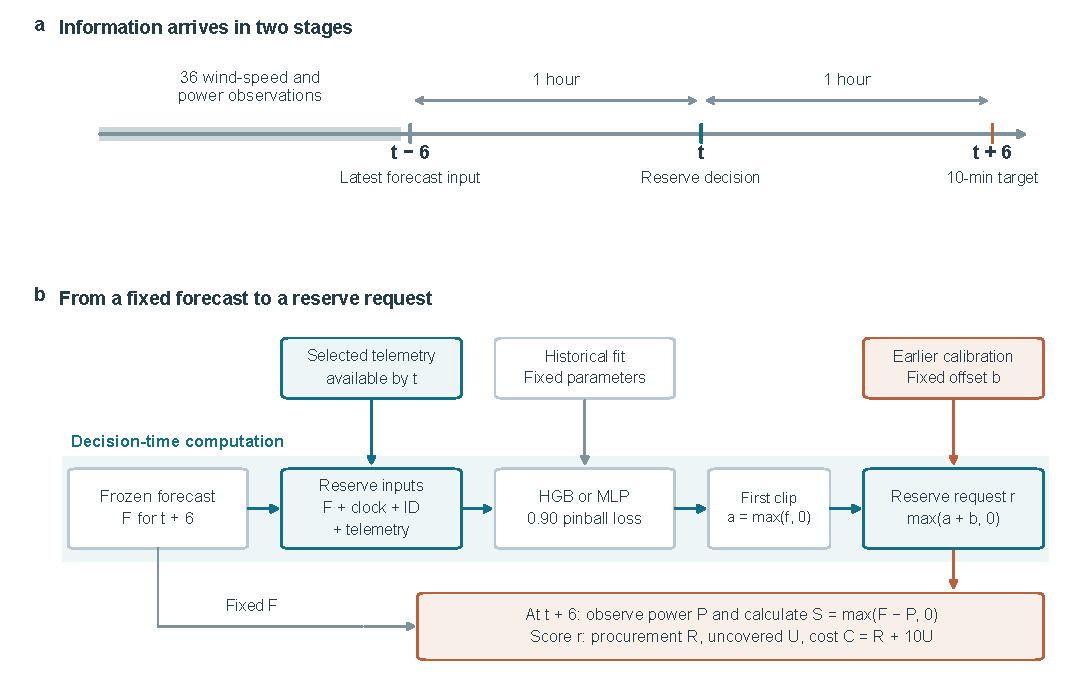
\includegraphics[width=\textwidth]{figures/v14/fig1_architecture.pdf}
\caption{Overall architecture and information timing. (a) On a ten-minute grid, the forecast uses 36 wind-speed and active-power observations ending at $t-6$. Reserve is requested at $t$ for the ten-minute target at $t+6$. The latest forecast input and the target are two hours apart; the reserve lead is one hour. The older history segment is schematic. (b) Available telemetry augments the forecast, clock and turbine identifier. The estimator output is clipped at zero, the signed historical offset is added, and the result is clipped again. Parameters and offsets remain fixed during evaluation. Future power enters shortfall and cost accounting only. This is a controlled information arrangement, not a measured communication delay.}
\label{fig:overview}
\end{figure*}

\subsection{Forecast commitment and shortfall loss}
Let $t$ denote the reserve decision time on a ten-minute grid, and let $i$ identify a turbine. The common forecast $F_{i,t}$ uses 36 wind-speed and active-power observations ending at $t-6$ to predict power at $t+6$. Thus, the reserve decision precedes the target by one hour, while the forecast target lies two hours after its latest input. The forecast remains fixed when the reserve inputs change. This controlled information arrangement separates the upstream forecast from the additional telemetry supplied at decision time. The target is one ten-minute interval. For its measured active power $P_{i,t+6}$, forecast shortfall is
\begin{equation}
 S_{i,t}=\max(F_{i,t}-P_{i,t+6},0).
\label{eq:shortfall}
\end{equation}

A reserve policy $m$ requests nonnegative reserve $r^m_{i,t}$ in kW. With a ten-minute interval $\Delta=1/6$ h, procured energy and uncovered shortfall are $R^m_{i,t}=\Delta r^m_{i,t}$ and $U^m_{i,t}=\Delta\max(S_{i,t}-r^m_{i,t},0)$. We evaluate their asymmetric decision loss and the associated event indicator as
\begin{equation}
 \begin{aligned}
 C^m_{i,t}&=R^m_{i,t}+\rho U^m_{i,t},\quad \rho=10,\\
 V^m_{i,t}&=\mathbf{1}\{S_{i,t}>r^m_{i,t}\}.
 \end{aligned}
\label{eq:loss}
\end{equation}

The penalty ratio makes an uncovered deficit more costly than procuring the same energy as reserve. Cost is expressed as a kWh-equivalent proxy per valid turbine interval; procurement and uncovered shortfall are expressed in kWh. For the corresponding unconstrained newsvendor decision, the expected loss is minimized at the conditional $(1-1/\rho)=0.90$ shortfall quantile. This relation motivates quantile regression for the reserve request \cite{koenker1978regression,soares2016}.

\subsection{Reserve estimators and historical offsets}
Each learned policy receives four common inputs: the point forecast, sine and cosine of time of day, and normalized turbine identifier. Telemetry configurations add measurements to these shared inputs. We use histogram gradient boosting (HGB) and a multilayer perceptron (MLP), both trained with the 0.90 pinball loss. HGB uses 100 boosting iterations and at most 15 terminal leaves. The MLP has two rectified linear hidden layers containing 64 and 32 units. Preprocessing is fitted on training data; complete settings are given in Supplementary Section S3.

Let $a^m_{i,t}=\max(f_m(x_{i,t}),0)$ denote the nonnegative raw reserve estimate for input vector $x_{i,t}$. A signed offset is calculated from historical shortfall residuals at calibration level $q$:
\begin{equation}
 \begin{aligned}
 b_{m,q}&=\operatorname{Quantile}^{\mathrm{higher}}_q
 \{S_{i,t}-a^m_{i,t}:(i,t)\in\mathcal D_{\rm cal}\},\\
 r^{m,q}_{i,t}&=\max(a^m_{i,t}+b_{m,q},0).
 \end{aligned}
\label{eq:offset}
\end{equation}

The $q$ value indexes residual-offset calibration, rather than a separately trained quantile model. The calibration grid contains $q=0.90,0.925,0.95,0.975,0.99$. The primary Hill of Towie comparison uses $q=0.95$; the secondary finite-family analysis uses $q=0.925$. Five fitted instances use seeds 201--205, with matched training samples across input configurations.

Figure~\ref{fig:decisionexample} illustrates this construction using a complete recorded day. The request follows the nonnegative estimator output with the same historical offset at every decision. Subsequent shortfalls reveal both covered and uncovered outcomes, while the offset grid shows the calibration choices made before evaluation.

\begin{figure*}[!t]
\centering
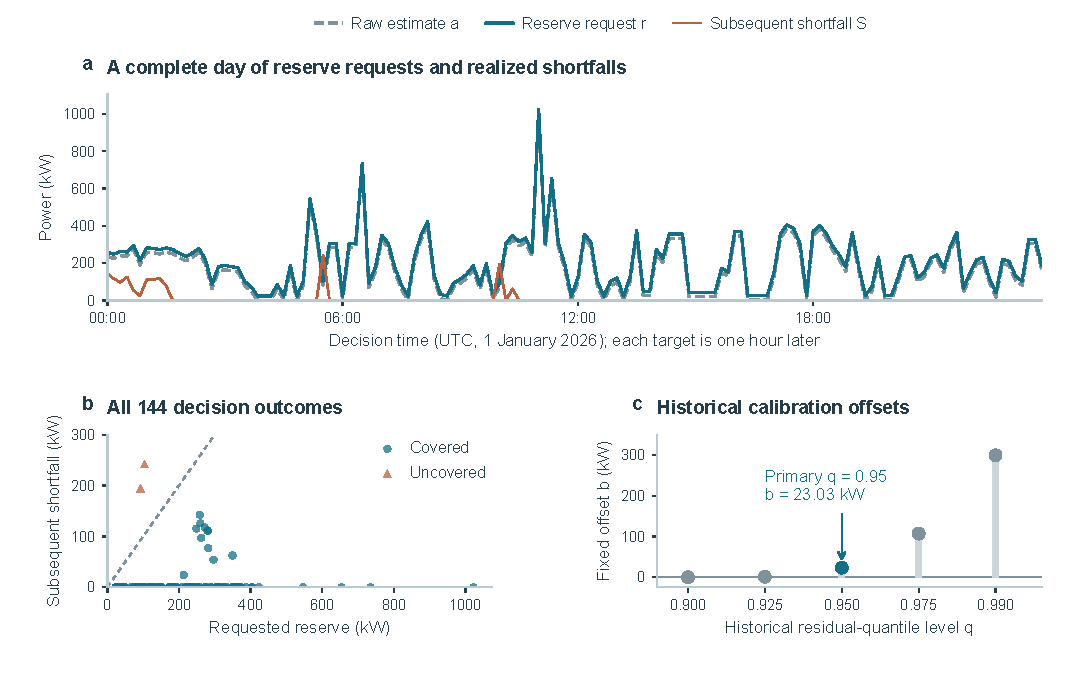
\includegraphics[width=\textwidth]{figures/v14/fig2_decision_example.pdf}
\caption{Reserve construction in a recorded day at Hill of Towie: turbine 1, 1 January 2026, P1/HGB, seed 201, $q=0.95$. (a) All 144 raw nonnegative estimates, final requests and subsequent shortfalls are retained. Shading marks shortfall above the request. The horizontal axis is decision time; each outcome belongs to the target one hour later. (b) Every request is paired with its realized shortfall. The dashed equality line separates covered circles from uncovered triangles; the two axes have different ranges to show the observed outcomes clearly. (c) The five stored historical residual offsets, with the primary $q=0.95$ offset highlighted. These are calibration choices, not confidence intervals or separately fitted quantile models.}
\label{fig:decisionexample}
\end{figure*}

\subsection{Fixed-reference requirements and resource order}
For candidate $m$ and fixed reference $b$, define relative mean-cost difference $D_C=\bar C_m/\bar C_b-1$. A rule is qualified if
\begin{equation}
 \begin{aligned}
 \operatorname{UCB}_{.95}(D_C)&\le 0.02,\\
 \max_s\operatorname{UCB}_{.95}(V_{m,s})&\le0.10,\\
 \max_s\operatorname{UCB}_{.95}(V_{b,s})&\le0.10.
 \end{aligned}
\label{eq:criteria}
\end{equation}

Here $s$ indexes the five fixed fits, and UCB denotes the upper bound from the simultaneous procedure below. The 2\% cost margin defines the accepted premium for input reduction. The event-rate cap applies to every fit of both candidate and reference. These declared comparison criteria assess cost and event frequency; procurement and uncovered-shortfall magnitude provide the accompanying action accounting.

Historical selection uses risk bounds and mean cost to choose the offset for each fitted recipe. Resource-minimal recipes are retained from the historically identified near-optimal set. The richer reference is selected from risk-qualified three-channel recipes on the same historical period. Both choices are then held fixed during subsequent evaluation.

For finite-family assessment, policies are ordered lexicographically by added telemetry channels, learned predictor passes and raw input width. Passing the fixed-reference criteria establishes sufficiency relative to that reference. A resource minimum within the registered finite family additionally requires exclusion of every strictly smaller candidate.

\subsection{Paired block inference}
We estimate uncertainty using 20,000 circular resamples of contiguous UTC weather days \cite{kunsch1989jackknife}. The primary block length is three days, with one-day and seven-day sensitivity analyses. The same day blocks are used for all paired policies and fits. Daily numerators and valid-record denominators are resampled together, then pooled to calculate interval-level means. A maximum standardized deviation gives an approximate simultaneous 95\% envelope for each declared comparison family. Studies and evaluation windows have separate families. Weather days are the sampling units, and the five fitted instances remain fixed. Supplementary Section S4 specifies the families and random seeds.

% Declare result floats before the study text to keep them close to the case studies.
\begin{figure*}[!t]
\centering
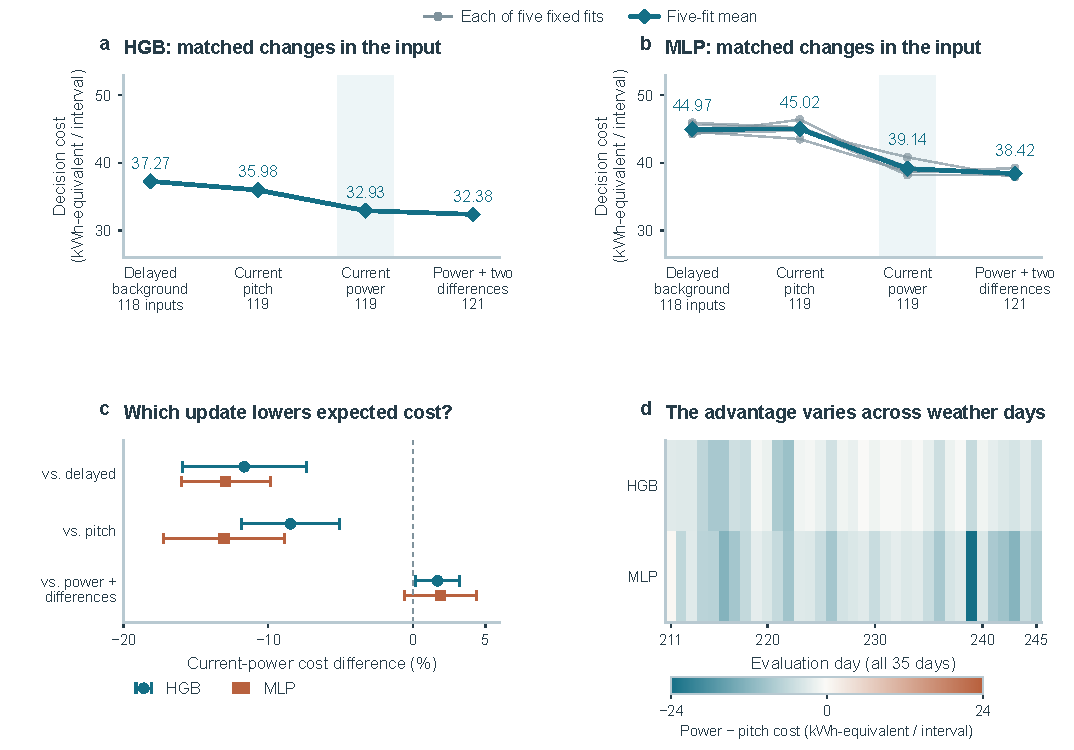
\includegraphics[width=\textwidth]{figures/v14/fig3_measurement.pdf}
\caption{The value of current measurements on a matched SDWPF population. (a), (b) Four input configurations share the same delayed background and evaluation rows. Thin lines connect each of the five fixed fits; diamonds and numbers show their means. Input counts include the four common inputs. (c) Relative current-power cost differences with stored approximate simultaneous 95\% intervals. Negative values favour current power. (d) Paired power-minus-pitch cost for every evaluation day, averaging the five fits. Blue denotes lower cost with power, and brown denotes higher cost. All 35 days and all 671,538 valid turbine intervals per fit are retained. The heatmap shows daily means.}
\label{fig:measurement}
\end{figure*}

\begin{figure*}[!t]
\centering
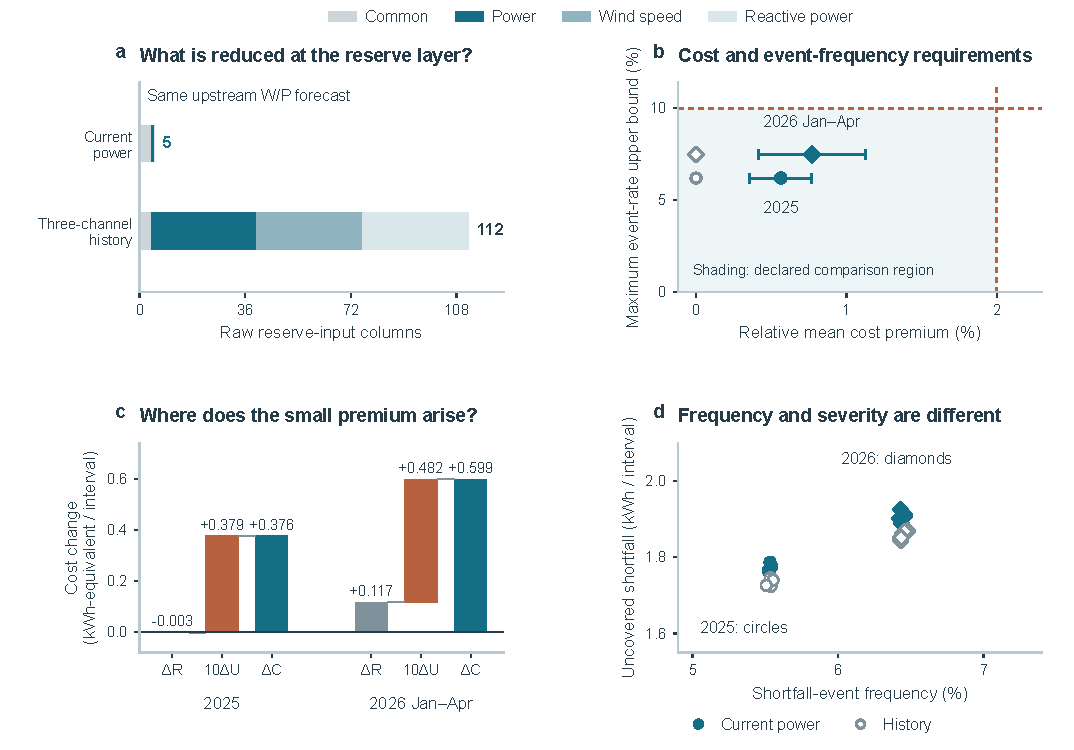
\includegraphics[width=\textwidth]{figures/v14/fig4_cross_year.pdf}
\caption{The cross-year trade-off from a compact reserve input. Both rules use HGB and $q=0.95$. (a) Input widths at the reserve layer, including four common inputs; the upstream forecast still uses wind-speed and power histories. (b) Filled markers show current-power relative mean cost and the maximum event-rate upper bound across five fits. Horizontal intervals are approximate simultaneous 95\% cost intervals. Open markers show the corresponding reference event bounds at zero self-relative cost. The shaded region marks the 2\% cost margin and 10\% event cap; years have separate inference families. (c) The cost premium decomposes as $\Delta C=\Delta R+10\Delta U$. The middle waterfall bar starts at $\Delta R$, and the final bar shows the total. (d) All five fit endpoints for each rule and period show event frequency alongside uncovered-shortfall magnitude. These points are descriptive, not confidence bounds.}
\label{fig:crossyear}
\end{figure*}

\begin{figure*}[!t]
\centering
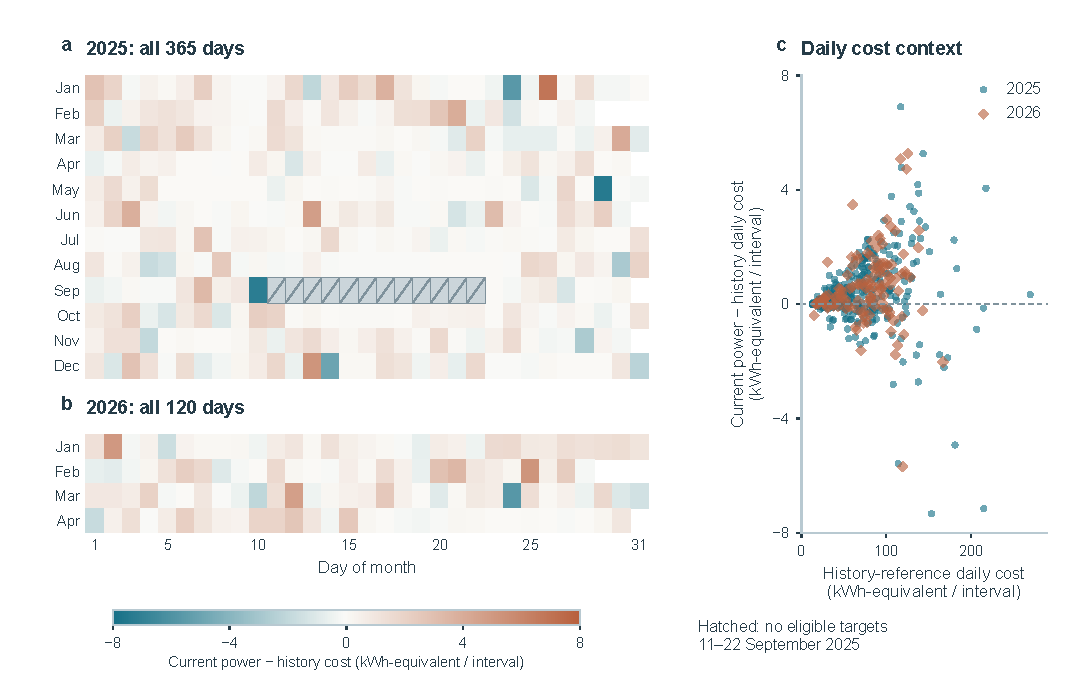
\includegraphics[width=\textwidth]{figures/v14/fig5_temporal.pdf}
\caption{Daily cost differences across the complete evaluation calendars. (a), (b) Each calendar cell shows the five-fit mean paired cost difference, current power minus history, using the same colour scale. Blue favours current power and brown favours history. All 365 dates in 2025 and 120 dates in January--April 2026 are retained. Gray cells with diagonal marks denote 11--22 September 2025, when no eligible targets were recorded; blank cells beyond a month's final day are not dates. (c) All valid daily differences are plotted against the reference's daily cost. These descriptive day-level views retain heterogeneous outcomes; window-level estimates pool valid-record numerators and denominators, with uncertainty reported in Fig.~\ref{fig:crossyear}.}
\label{fig:temporal}
\end{figure*}

\section{Study Design}
\label{sec:design}

\subsection{Matched current-measurement comparison}
The first study uses the public SDWPF dataset, which contains 134 turbines with ten-minute records \cite{zhou2024sdwpfdata}. A common point forecaster is fitted on days 1--90. Reserve models are fitted on days 136--175, offsets are calibrated on days 176--192, and historical assessment uses days 193--210. Evaluation uses days 211--245.

The delayed background contains 118 raw columns: four shared forecast and clock inputs, 36 slots each for wind speed, active power and reactive power, and six summaries of available power history. Its most recent six slots are masked to represent a one-hour delay. The analysis does not search backward for replacement observations.

Two matched updates append either current active power or current mean blade pitch to this background. Both therefore use 119 raw columns. An augmented-power condition also adds current power, forecast-minus-current power and current-minus-last-arrived power. This 121-column configuration tests the contribution of two derived power features. All updates refer to the same decision time.

The evaluation population requires finite future active power, current active power and current pitch. Every configuration uses the same 671,538 turbine intervals per fitted instance across 35 days. Zero and negative active power are retained. Training and calibration use finite future targets. Each fit uses 360,000 matched training rows and the historical calibration level $q=0.925$ for the current-power update.

\begin{table}[!t]
\caption{Chronological study design. Evaluation counts are valid turbine intervals per fixed fit.}
\label{tab:design}
\centering
\footnotesize
\begin{tabularx}{\columnwidth}{lXX}
\toprule
Stage & SDWPF, 134 turbines & Hill of Towie, 21 turbines \\
\midrule
Point forecast & Days 1--90 & 2023 H1 \\
Reserve fit & Days 136--175 & 2023 H2 \\
Offset calibration & Days 176--192 & 2024 H1 \\
Historical selection & Days 193--210 & 2024 H2 \\
Evaluation & Days 211--245, 671,538 intervals, 35 days & 2025: 1,059,248 intervals, 365 days; 2026 Jan--Apr: 361,326 intervals, 120 days \\
\bottomrule
\end{tabularx}
\end{table}

\subsection{Hill of Towie historical selection and subsequent evaluation}
The second study uses the public Hill of Towie dataset. It contains 21 turbines with UTC timestamps marking ten-minute period ends \cite{clerc2026towie}. A common point forecaster is trained on January--June 2023 using up to 120,000 samples. Reserve rules are fitted on July--December 2023 with 360,000 matched samples per seed. Offset calibration uses January--June 2024, and historical selection uses July--December 2024. Labels are required to mature before the next forecasting stage begins.

The pitch-withheld input family contains Common and all 21 nonempty combinations of wind speed, active power and reactive power at history lengths 1, 6 and 36. HGB and MLP are paired with these subsets. A power-persistence rule and five historical offset levels produce 225 registered policies.

Historical selection retains the HGB rule that adds current active power and the HGB reference using 36-step histories of all three channels. Their resource tuples are $(1,1,5)$ and $(3,1,112)$. The tuples count additional telemetry channels, learned predictor calls and raw reserve-input columns. Both rules share the forecast and common inputs. The reported input reduction therefore applies to the reserve layer, not the upstream forecast.

The two selected rules and the common point forecaster are evaluated on the full 2025 year. The same fitted parameters and offsets are then used for January--April 2026. The latter period includes the documented Dynamic Yaw campaign; all prespecified turbines and times remain in the evaluation. The same future-target definition and mask are applied to both rules.

The secondary finite-family analysis evaluates the registered calibration grid in 2025. The fixed-reference comparison and the secondary minimum-identification analysis answer different questions, so their calibration levels are reported separately.

\section{Case Studies}
\label{sec:results}

\subsection{Current power and pitch carry different decision value}
With the same delayed telemetry background, adding current active power reduced reserve decision cost relative to adding current pitch. Both measurements add one raw input at the same decision time, while retaining the common forecast commitment. In the 134-turbine comparison, HGB cost was 8.47\% lower with current power than with current pitch (approximate simultaneous 95\% interval, $[-11.88,-5.07]\%$). MLP gave a reduction of 13.05\% ($[-17.22,-8.88]\%$). The agreement across estimators shows that the contrast is not specific to one fitting procedure (Fig.~\ref{fig:measurement}).

Current power also reduced HGB cost by 11.66\% relative to the delayed-only background ($[-15.94,-7.37]\%$). Adding two power-derived differences to the current-power update improved cost further. The current-power-only rule had 1.70\% higher cost than that augmented input ($[0.16,3.23]\%$). The power measurement therefore accounts for a substantial cost reduction before these derived features are added. The lower mean cost did not establish a uniform reduction in uncovered shortfall across all five fits.

Figure~\ref{fig:measurement}(a), (b) shows the paired changes across all four input configurations, including the additional gain from the two power-derived features. The daily comparison in Fig.~\ref{fig:measurement}(d) retains the variation across shared weather days. Mean procurement and uncovered shortfall are both lower with the power update than with pitch; complete endpoint accounting is reported in Supplementary Table S2.

\subsection{A compact reserve input retains performance across years}
The historically selected rule using current power met the fixed-reference requirements in both subsequent periods. It adds one telemetry channel to the four common inputs, giving five raw columns. The reference uses three 36-step channel histories and 112 raw columns in total. Both retain the same upstream forecast, so this reduction concerns the reserve input supplied after forecast issuance.

In the 2025 evaluation, the current-power rule had mean cost 67.0204 kWh-equivalent per valid interval, compared with 66.6444 for the three-channel reference. The relative difference was 0.5641\% ($[0.3575,0.7708]\%$). Maximum event-rate upper bounds across fits were 6.2025\% and 6.2004\%, respectively. The cost bound remained below the 2\% margin, and both rules met the 10\% event-rate limit.

The fitted models and historical offsets were retained for the January--April 2026 evaluation. The current-power rule had a mean cost of 78.4144 kWh-equivalent per valid interval, versus 77.8157 for the reference. Its relative cost difference was 0.7694\% ($[0.4128,1.1260]\%$). Maximum event-rate upper bounds were 7.4846\% and 7.4886\%, respectively. Both requirements also held with one-day and seven-day block lengths. The documented Dynamic Yaw operating period remained in the evaluation. Figure~\ref{fig:crossyear} places the input reduction alongside the two performance requirements and the resulting cost composition.

The cost decomposition explains the price of this input reduction (Fig.~\ref{fig:crossyear}(c)). In 2026, the current-power rule requested 59.3417 kWh per interval, compared with 59.2249 kWh for the reference. Mean uncovered shortfall was 1.9073 and 1.8591 kWh, respectively. Their similar event rates therefore accompanied a small difference in shortfall magnitude, also visible across the individual fits in Fig.~\ref{fig:crossyear}(d). The compact rule retained the specified cost and event-frequency performance with this explicit trade-off. Supplementary Table S3 gives the complete endpoint means.

\subsection{Daily differences reveal the variation behind window means}
Figure~\ref{fig:temporal} places the window-level comparison in its chronological context. The full calendars show days on which current power costs more or less than the history reference. Plotting these differences against the reference's daily cost makes their size visible within the operating conditions actually encountered. The twelve September days without eligible targets remain marked as missing. All other dates use the same valid-target population as the primary comparisons.

\subsection{The registered family admits a resource minimum in 2025}
A separate 2025 analysis identified a sufficient resource-minimal rule at offset level $q=0.925$. Its mean cost was 65.7392 kWh-equivalent per valid interval, and its maximum event-rate upper bound was 9.7699\%. All 15 strictly smaller registered candidates were excluded: two by the risk condition and 13 by paired cost comparisons (Supplementary Table S4). This family-wide result concerns the $q=0.925$ rule. The cross-year comparison above concerns the historically selected $q=0.95$ rule; minimum identification was not repeated in 2026.

\section{Discussion}

The two studies support evaluating telemetry at the decision layer where it is used. A forecast can summarize a substantial history without making every subsequent measurement redundant. In the matched study, current power reduced cost even when its two derived differences were removed. In the cross-year study, current power and the shared forecast supported a reserve rule with a much smaller raw input set. The common lesson is that input requirements depend on the forecast already available and the decision loss imposed downstream.

This finding complements turbine-level probabilistic forecasting \cite{gilbert2020} and forecast-error models for reserve sizing \cite{bruninx2014}. Those studies improve the uncertainty description available for operation. Here, the forecast commitment remains unchanged while the additional reserve inputs vary. The resulting comparison identifies an opportunity to simplify the interface between forecasting and reserve estimation, without redesigning the forecasting model.

The cost and event-rate criteria give that simplification a concrete meaning. They allow a small cost premium in exchange for fewer reserve inputs. The shortfall decomposition matters because nearly identical event frequencies can conceal different deficit magnitudes. Reporting procurement and uncovered energy alongside event rate therefore reveals the operating trade-off accepted by the reduced interface.

Decision-focused feature selection already establishes the importance of downstream cost \cite{munoz2020featuredriven,serrano2024featureselection}. Our results extend that perspective to additional measurements arriving after a common forecast. Matching the update width and retaining the selected rules across later periods make this a test of a specified telemetry interface. The finite-family minimum further shows how an input-reduction claim can be tested against smaller alternatives, provided the family and calibration level are explicit.

The resulting simplification applies to the reserve learner's inputs. The upstream forecast continues to use wind and power history, and raw input width does not quantify communication or computing savings. The present loss measures turbine-level procurement and uncovered shortfall. Applying the same interface to a delivered reserve service would additionally require network constraints and settlement rules. Such an evaluation would determine whether the observed input trade-off remains attractive for a particular operating system.

\FloatBarrier
\section{Conclusion}

This paper evaluated the additional telemetry needed for reserve decisions under an unchanged wind power forecast. Current power reduced decision cost relative to a matched current-pitch update under both tested estimators. A historically selected current-power rule then met the specified cost and event-rate requirements in two subsequent evaluation windows. The results support a compact reserve input interface whose value is assessed through the resulting procurement and shortfall trade-off.

\section*{Acknowledgment}
OpenAI Codex and Google Gemini assisted with drafting and language revision across the Abstract, Introduction, Methods, Results, and Discussion. Codex assisted with the vector diagrams and plotting code. All plotted data and numerical values come from the study records.
\bibliographystyle{IEEEtran}
\IEEEtriggeratref{8}
\bibliography{references}
\end{document}
